% Structure
%    intro
%    purpose
%    (maybe) helix coords (appendix?)
%    general barrel/endcap cylindrical structure
%    walkthrough of the systems, from inner to outer, discussing why they are there and their basic purpose
%    Then split off into sections for the individual subsystems

    %Discussion of radiation hardness?
    %Things in the endcap suffer from more radiation exposure than things in the barrel
    %    (you should be able to show this from the basic kinematics of the particle beams. most energy is deposited in parallel to the beams, not orthogonal to them)
    %things closer to the IR suffer more than things further away (literally just the inverse-square law)

    %Discussion of using cheaper things as you get further out? (better angular resolution with lower spatial resolution, larger area to be covered, less risk from radiation damage)


\chapter{ATLAS} 
    % Intro
    Production of new physics and particles is of little use without the ability to observe said physics.
    Herein lies the purpose of ATLAS.
    One of the two general purpose detectors at the LHC, construction of the ATLAS detector was completed on October 4, 2008.
    ATLAS is among the largest particle detectors ever built, measuring 46m long with a 25m diameter, and weighing in at 7,000 tonnes \cite{atlas_website}.

    \begin{figure}[h]
        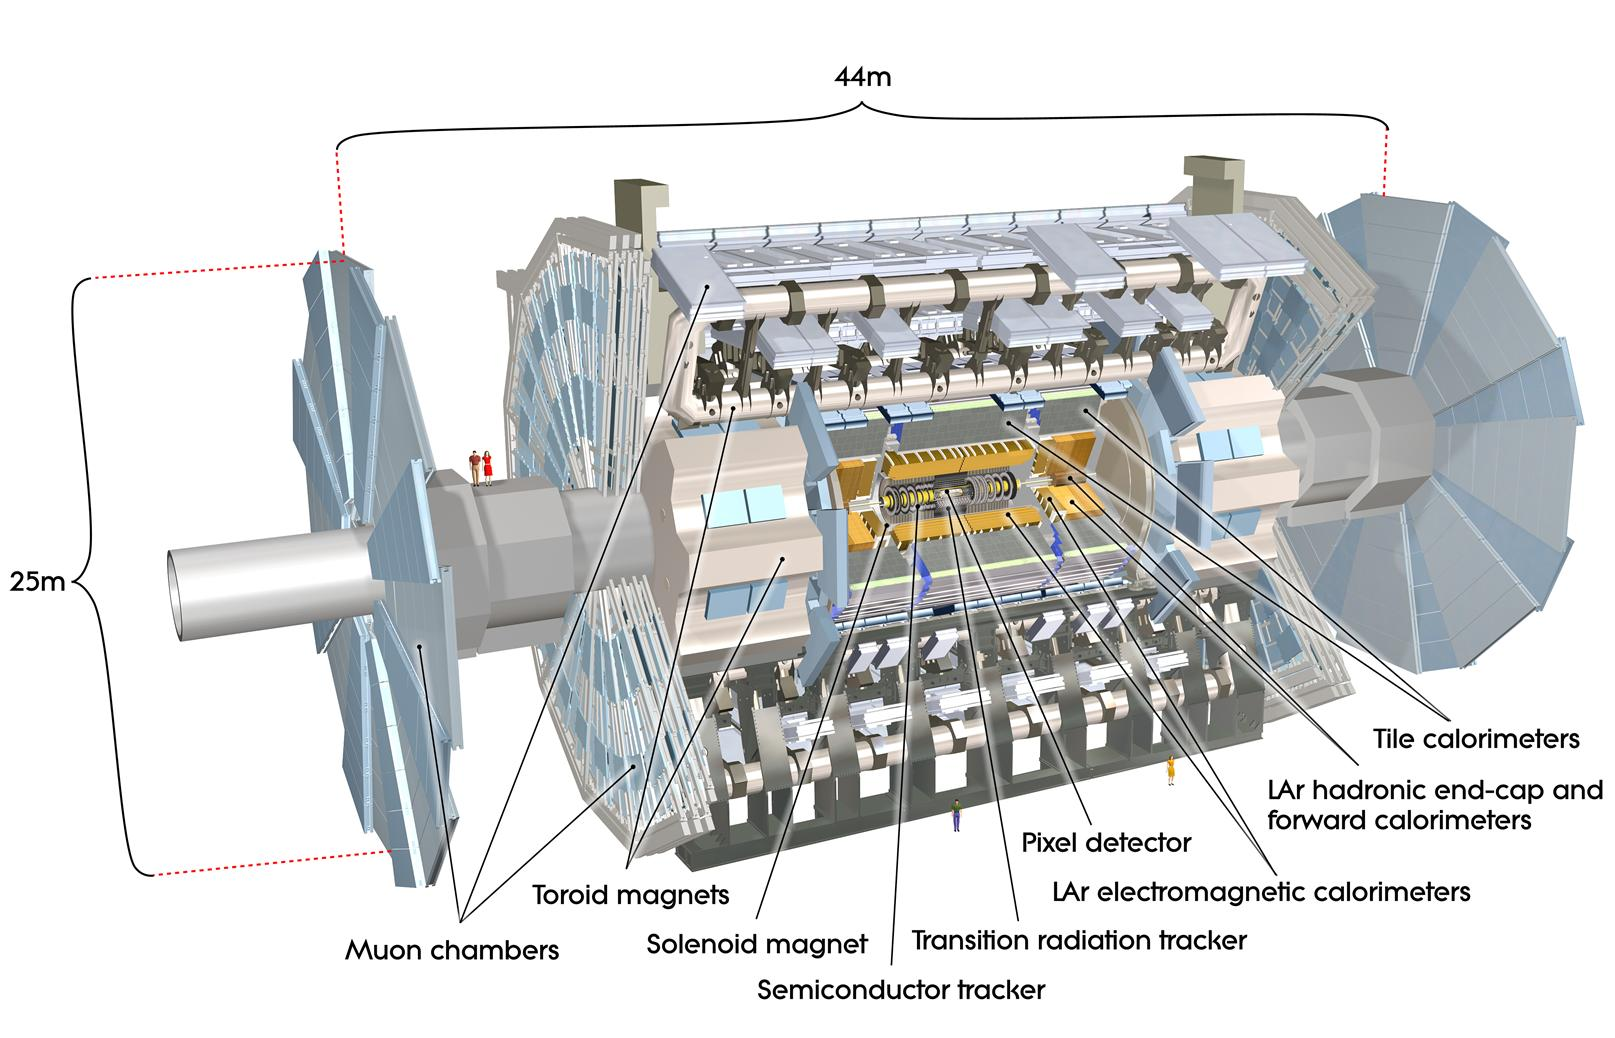
\includegraphics[width=\linewidth,height=\textheight,keepaspectratio]{atlas/atlas_xsec}
        \caption{Cutaway view of the ATLAS detector \cite{Pequenao:1095924}}
        \label{fig:atlas_xsec}
    \end{figure}


    % Purpose
    The overall function of the ATLAS detector is to accurately record the physical properties of the particle interactions which take place in the detector's Interaction Region (IR).
    Most of the particles of interest are extremely short-lived, and so their properties cannot be measured directly.
    Instead, these particles must be reconstructed based on detection of their decay products.
    Accurate reconstruction of these original particles is critically dependent on measuring, as precisely as possible, the physical properties of these decay products.
    To be more specific, ATLAS is designed to record the paths and decay showers of the particles which pass through the detector, in order to determine their mass, energy, momentum, and electric charge.

    \begin{figure}
        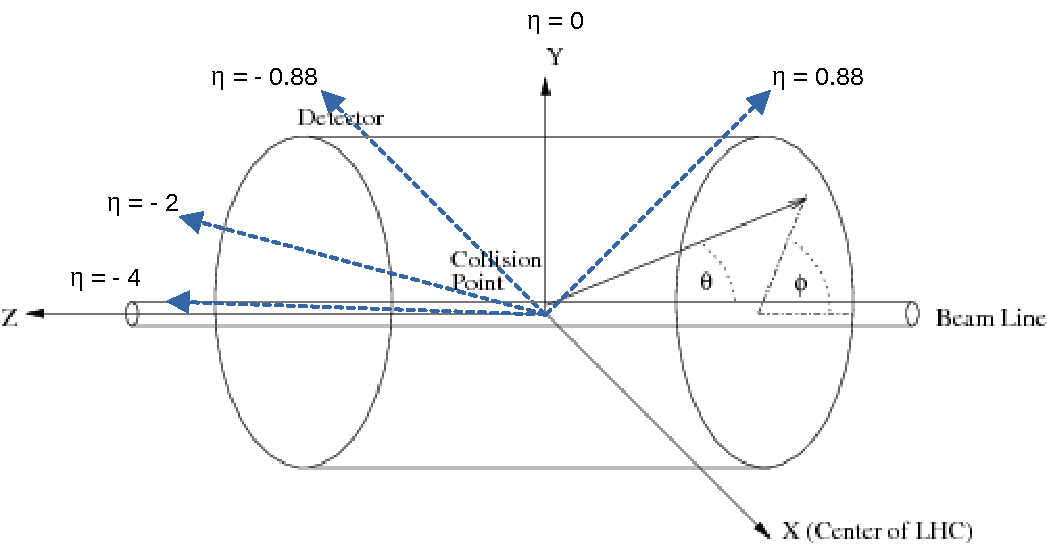
\includegraphics[width=\linewidth,height=\textheight,keepaspectratio]{atlas/atlas_coords}
        \caption{Illustration of the cylindrical coordinate system used in ATLAS \cite{Schott:1699952}}
        \label{fig:atlas_coords}
    \end{figure}

    % General barrel/endcap cylindrical structure
    In order to measure all required properties, ATLAS is divided into many different subsystems.
    Each of these subsystems has a very different design and objective, but they are all constructed with roughly the same overall cylindrical geometry.
    The reason for this design is simple kinematics.
    The LHC particle beams cross with no initial transverse momentum, which means particles are ejected without preference in the radial angle $\phi$.
    Furthermore, the extremely high longitudinal momentum of the beams results in many particles continuing along a highly ``forward" (parallel to the beampipe) trajectory.
    These two properties lead naturally to a radially symmetric detector which is elongated in the forward direction; a cylinder centered on the beam axis.
    To accommodate this geometry, the various sub-detectors of ATLAS are generally split into two distinct parts, called ``barrels" and ``endcaps".
    The barrels are a series of radially symmetric cylindrical shells, concentric about the beampipes, meant to detect particles moving primarily in the transverse direction.
    In turn, the endcaps are a series of flat, circular plates, stacked one behind the next along the beampipes, intended to detect more forward particles.
    Nearly all of the sub-systems described below will have both barrel and endcap components.

    % Walkthrough of the systems, from inner to outer, discussing why they are there and their basic purpose
    The various detector subsystems can be broken up into three primary groups, based on their purpose.
    The subsystems are arranged in concentric shells, each group further from the IR than the last.
    Moving out from the interaction region, the subsystems can be classified as belonging to the Inner Detector, the Calorimeter System, and the Muon Spectrometer.
    The first of these, located as close in $r$ and $z$ as possible, is the Inner Detector system.
    The Inner Detector is designed to provide momentum measurement, vertexing, and electron identification.
    It must be located so close to the interaction region in order to permit detection of short lived particles like b-quarks and tau leptons \cite{id_tdr}.
    Following immediately behind (endcap) and around (barrel) the Inner Detector is the collection of sensors comprising the Calorimetry system.
    These sensors are purpose-built to measure the energy of incoming particles and also provide supplementary tracking information for particle trajectories.
    Their location between the IR and Muon System is based on the fact that calorimeters function by absorbing all of a particle's energy, thereby stopping them.
    Since their function necessarily stops particles, they must be placed outside the range of the tracking system, as otherwise the trackers would never see particles.
    The Muon system however functions best when only muons traverse it, and so the calorimeters are intentionally placed between the IR and the Muon Spectrometer in order to shield the Muon system from unwanted hadrons.
    Finally, at the outer edge of ATLAS, is the Muon Spectrometer, which has been built to measure the momentum of muons leaving the detector volume.

% Then split off into sections for the individual subsystems
\section{Inner Detector} \label{sec:inner_detector}
    % Purpose of subsystem
    % Basic specs
    % What mechanism is used to achieve this purpose
    % What are the individual detectors and how do they contribute to this goal
    
    The Inner Detector system is intended to provide measurement of particles' momentum, provide vertex information, and help in identifying electrons.
    The way it achieves these goals is primarily through a series of very high resolution tracking sensors, which are used to trace out the paths that particles traverse as they leave the IR. 
    Momentum and charge measurement is facilitated by using a solenoid magnet to encompass the entire Inner Detector with a 2T axial magnetic field.
    This field bends the high-momentum charged particles into a helical trajectory, allowing their momentum, mass, and charge to be determined from the shape of the particle's path.
    The entire ID system, consisting of three independent detectors, measures 5.3 m in length and 2.5 m in diameter, and is able to provide accurate tracking within $|\eta| < 2.5$ \cite{id_tdr}.
    From the innermost to outermost, the sub-detectors are the Pixel Detector, the Semiconductor Tracker (SCT), and the Transition Radiation Tracker (TRT).
    The Pixel Detector and SCT together are responsible for high resolution tracking of particle trajectories.
    Further from the IR, the TRT provides more particle tracking capability at lower resolution (but higher statistics), as well the ability to help distinguish electrons. 

    \begin{figure}[h]
        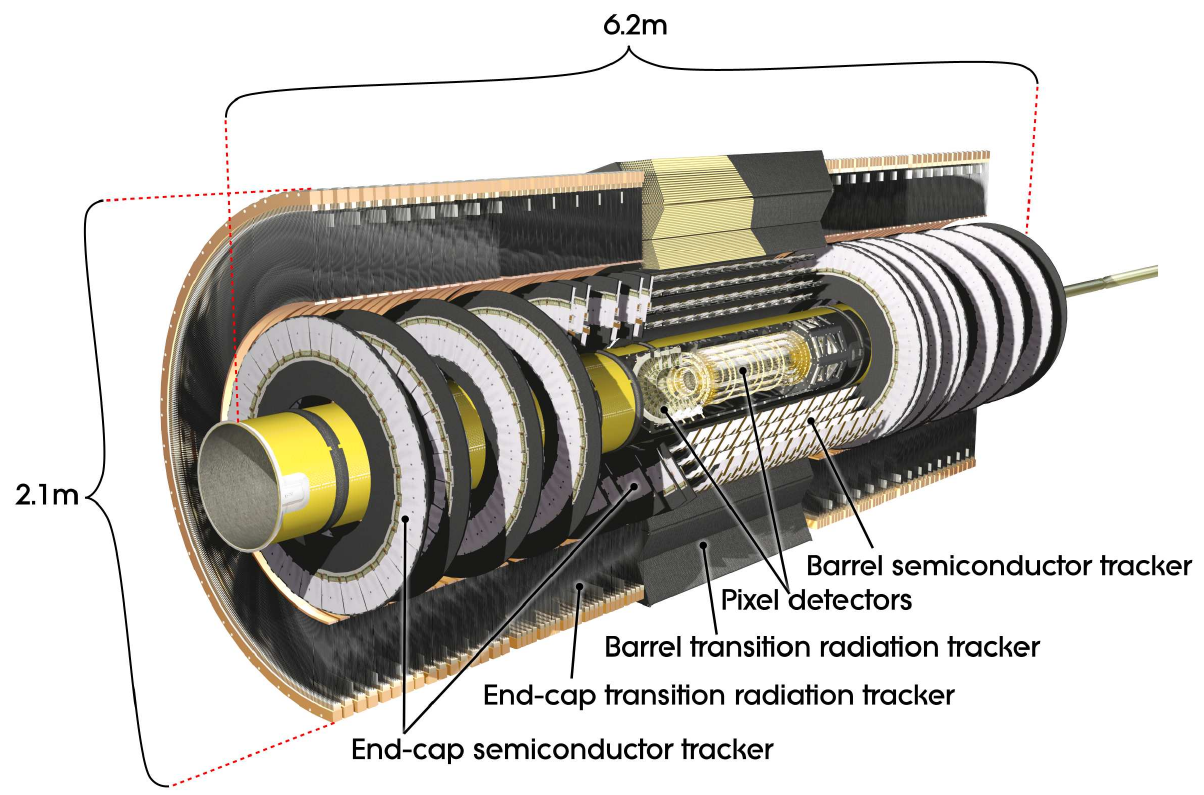
\includegraphics[width=\linewidth,height=\textheight,keepaspectratio]{atlas/inner_detector_xsec}
        \caption{Cutaway view of the Inner Detector sub-system \cite{atlas_tdr}}
        \label{fig:inner_detector_xsec}
    \end{figure}

    \begin{table} \centering
\caption{General specifications of Inner Detector modules \cite{atlas_tdr} \cite{insertable_Blayer}.}
\label{tab:ID_specs}
\begin{tabular}{ |l l|l|l| }
    \hline
    \textbf{Item}                   & &       \textbf{Radial extension (mm)} & \textbf{Length (mm)} \\
    \hline
    \textbf{Overall ID envelope}    & &         \textbf{0 < R < 1150}        &\textbf{0 < |z| < 3512} \\
    Beam-pipe                       & &            29 < R < 36    & \\
    \hline

    \textbf{IBL}          &  Overall envelope  &  31.0 < R < 40.0          &             \\    
                          &  Sensitive barrel  &  <R> = 25.7               &  |z| < 332 \\    
    &&&\\
    \textbf{Pixel}        &  Overall envelope  &  45.5 < R < 242           &  0 < |z| < 3092 \\
    3 cylindrical layers  &  Sensitive barrel  &  50.5 < R < 122.5         &  0 < |z| < 400.5 \\
    2 × 3 disks           &  Sensitive end-cap &  88.8 < R < 149.6         &  495 < |z| < 650 \\
    &&&\\
    \textbf{SCT}          &  Overall envelope  &  255 < R < 549 (barrel)   &  0 < |z| < 805 \\
                          &                    &  251 < R < 610 (end-cap)  &  810 < |z| < 2797 \\
    4 cylindrical layers  &  Sensitive barrel  &  299 < R < 514            &  0 < |z| < 749 \\
    2 × 9 disks           &  Sensitive end-cap &  275 < R < 560            &  839 < |z| < 2735 \\
    &&&\\
    \textbf{TRT}          &  Overall envelope  &  554 < R < 1082 (barrel)  &  0 < |z| < 780 \\
                          &                    &  617 < R < 1106 (end-cap) &  827 < |z| < 2744 \\
    73 straw planes       &  Sensitive barrel  &  563 < R < 1066           &  0 < |z| < 712 \\
    160 straw planes      &  Sensitive end-cap &  644 < R < 1004           &  848 < |z| < 2710 \\
    \hline
\end{tabular} \end{table}



    \subsection{Pixel Detector and Semiconductor Tracker}
        % purpose
        As the very first detector elements that any particles leaving the interaction region will encounter, the Pixel Detector and SCT face a precarious dilemma.
        On the one hand, they must be able to accurately track the path of all ionizing particles emerging from the IR at high resolution (see table \ref{tab:ID_resolution}).
        On the other hand, any disturbance they introduce to particle trajectories will distort the measurement of every other detector in ATLAS.
        Add to this that these detectors face the highest radiation flux of any system simply by their proximity to the IR, forcing usage of very radiation-hard material design.
        For these reasons, the Pixel Detector and SCT use top-of-the-line silicon semiconductor diode technology, which can be made both extremely thin and sensitive. 
        This means that particles only deposit a small fraction of their energy into the detector material, and yet that small deposition is enough to accurately record their passage.
        With three layers of the Pixel Detector and four of the SCT, any particle leaving the IR crosses at least seven detector layers, yet continues on with a mostly unchanged trajectory.

        \begin{table}[] \centering \footnotesize
\caption{Resolution of the various Inner Detector Modules \cite{id_tdr}\cite{insertable_Blayer}.}
\label{tab:ID_resolution}
\begin{tabular}{|l|l|l|l|l|l|}
\hline
\textbf{System} & \textbf{Position} & \textbf{ Area }                 & \textbf{ Resolution }   & \textbf{ Channels } & \textbf{$\eta$} \\
\textbf{}       & \textbf{        } & \textbf{(m\textsuperscript{2})} & \textbf{\sigma($\mu$m)} & \textbf{ ($10^6$) } & \textbf{Coverage} \\
\hline
Pixels         & 1 insertable barrel layer & 0.38      & $R\phi$ = 50, z = 250    & 13.2           & $\pm 3  $       \\
               & 1 removable barrel layer  & 0.2       & $R\phi$ = 12, z = 66     & 16             & $\pm 2.5$       \\
               & 2 barrel layers           & 1.4       & $R\phi$ = 12, z = 66     & 81             & $\pm 1.7$       \\
               & 4 end-cap disks           & 0.7       & $R\phi$ = 12, R = 77     & 43             & 1.7-2.5         \\
               & on each side              &           &                          &                &                 \\
Silicon strips & 4 barrel layers           & 34.4      & $R\phi$ = 16, z = 580    & 3.2            & $\pm 1.4$       \\
               & 9 end-cap wheels          & 26.7      & $R\phi$ = 16, R = 580    & 3.0            & 1.4–2.5         \\
               & on each side              &           &                          &                &                 \\
TRT            & Axial barrel straws       &           & 170 (per straw)          & 0.1            & $\pm 0.7$       \\
               & Radial end-cap straws     &           & 170 (per straw)          & 0.32           & 0.7–2.5         \\
               & 36 straws per track       &           &                          &                &                 \\
\hline
\end{tabular} \end{table}


        Semiconductor diode detectors function by exploiting the properties of semiconductor p-n junctions.
        These particular detectors are made using silicon.
        Silicon has four valence electrons, so a pure silicon crystal lattice will have its valence band perfectly filled, leading to a very stable structure.
        A pure semiconductor crystal lattice (in this case, silicon) can have impurities intentionally introduced to it through the process of doping.
        Doping the lattice with an element possessing only three valence electrons (e.g. Boron) will result in a number of gaps in the valence band (called ``holes").
        In such a situation, known as p-type doping, the lattice will accept additional electrons to fill these holes, which will lead to an excess of negatively charged ions.
        Conversely, an element with five valence electrons can be introduced for doping, leading to an excess of electrons in the valence band.
        Known as n-type doping, such an excess results in a lattice with a propensity for shedding these excess valence electrons, which in turn leads to an excess of positive ions.
        A p-n junction can be produced by taking a single silicon wafer and n-type doping one half, while p-type doping the other.
        The junction where the separately doped halves meet will then see a transfer of excess valence electrons moving from the n-type side to fill the holes of the p-type side, as illustrated in figure \ref{fig:pn_junction}

        \begin{figure}
            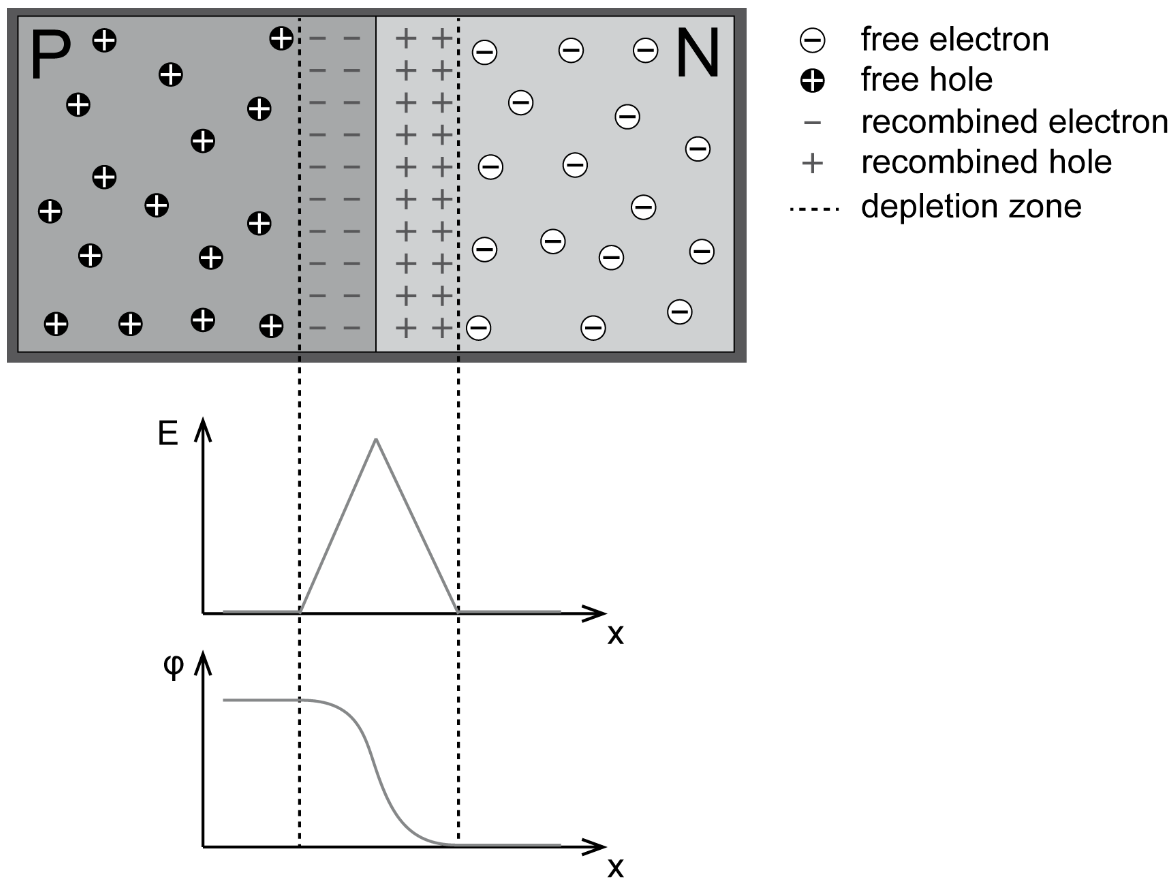
\includegraphics[width=\linewidth,height=\textheight,keepaspectratio]{atlas/pn_junction}
            \caption{Representation of a p-n junction, its depletion region, and the electric field and potential across its surface \cite{Havránek:2317324}}
            \label{fig:pn_junction}
        \end{figure}

        As the excess ``donor" electrons migrate to fill the ``acceptor" holes, the area around the junction has its valence band filled, creating an area called the ``depletion zone".
        Though the depletion zone has a filled valence band, it has done so at the cost of ionization; an excess of electrons now populates the p-type side, with an equal number of positive ions remaining on the n-type side.
        The depletion zone grows larger until the migration of holes and electrons is balanced by the electric potential created through this ionization.
        When equilibrium is achieved, the lattice is left with an electric potential which monotonically decreases from the n-type to the p-type side, and which spans the full width of the depletion zone (refer again to figure \ref{fig:pn_junction}).
        If a voltage is applied across the semiconductor, the width and potential difference of the depletion region can be altered.
        If the voltage is applied with the positive end of the difference at the p-type side, then the semiconductor is said to be ``forward biased", and the depletion region will become smaller (and with a high enough voltage can be eliminated entirely).
        If the positive end of the voltage difference is applied to the n-type side though, the semiconductor becomes ``reverse biased", and the depletion region and potential difference across the junction will grow larger \cite{wiley_radiation_detection}.
        In this reverse-biased state, the electric potential of the p-n junction becomes very effective at rapidly sweeping excess ions from the depletion region off to the edges of the semiconductor wafer, and it is this mechanism which the ATLAS semiconductor detectors exploit in order to detect particles.

        Ionizing radiation is any particle that interacts electromagnetically, which means either photons or any particle with electric charge.
        When ionizing radiation passes through an element of the Pixel Detector or SCT, it will momentarily separate electrons from their nuclei in the silicon lattice.
        Normally, such separated ions would just recombine in a matter of moments.
        Because of the electric potential in the depletion region though, these ions are further separated, and swiftly arrive at opposite ends of the semiconductor wafer.
        The electrical contacts responsible for biasing the semiconductor are then responsible for collecting these separated ions, which will cause a sudden jump in the circuit's current.
        The electric current through these semiconductor detectors is closely monitored, and these spikes are used to identify the passage of a particle through the semiconductors.

    \subsection{Transition Radiation Tracker (TRT)}
            While the Pixel Detector and SCT focus on quality over quantity in their tracking, the TRT serves to take the opposite approach.
            The TRT has a resolution much lower than that of either the Pixel or SCT (table \ref{tab:ID_resolution}).
            But where the Pixel and SCT combined only manage about seven recorded hits per particle, the TRT achieves around 36.
            High statistics then are able to offset the TRT's lower resolution per hit, overall achieving a similar uncertainty on its track measurements.
            Such measurement needs to be accomplished under the same restrictions faced by the earlier trackers though.
            Namely, that it must obtain these measurements while causing minimal deviation in particle trajectory and also tolerating heavy radiation exposure over time.
            These challenges and goals are addressed in the TRT's composition, using a detector technology known as ``proportional drift tubes".

            Proportional drift tubes, often referred to as ``straws", function in a similar way to semiconductor diode detectors, but using a gas instead of a doped semiconductor.
            The primary component of a drift tube is a cylinder filled with a gas mixture.
            In the TRT, these cylinders are 4 mm in diameter, filled with a mixture of 70\% Xenon, 27\% CO\textsubscript{2}, and 3\% O\textsuperscript{2}.
            Ions are produced in this mixture when ionizing radiation passes through it.
            As in the semiconductor diode detectors, these ions are collected by applying an electric field through the ionization medium in order to sweep ions away into external circuitry for readout.
            In a drift tube this is accomplished by maintaining an electric potential between the tube wall and a conductive wire running through the cylinder axis \cite{drift_chambers}.
            %NOTE: do I need to mention avalanche multiplication?
            The wall of the tube acts as the positively charged anode to collect electrons produced by the ionization, while the axial wire is kept at high electrical potential to act as the cathode.
            In the TRT, the cathode wall is made of aluminium and the 30 $\mu$m diameter anode wire of gold-plated tungsten. \cite{trt_design}

            \begin{figure}
                \begin{subfigure}{.48\textwidth}
                    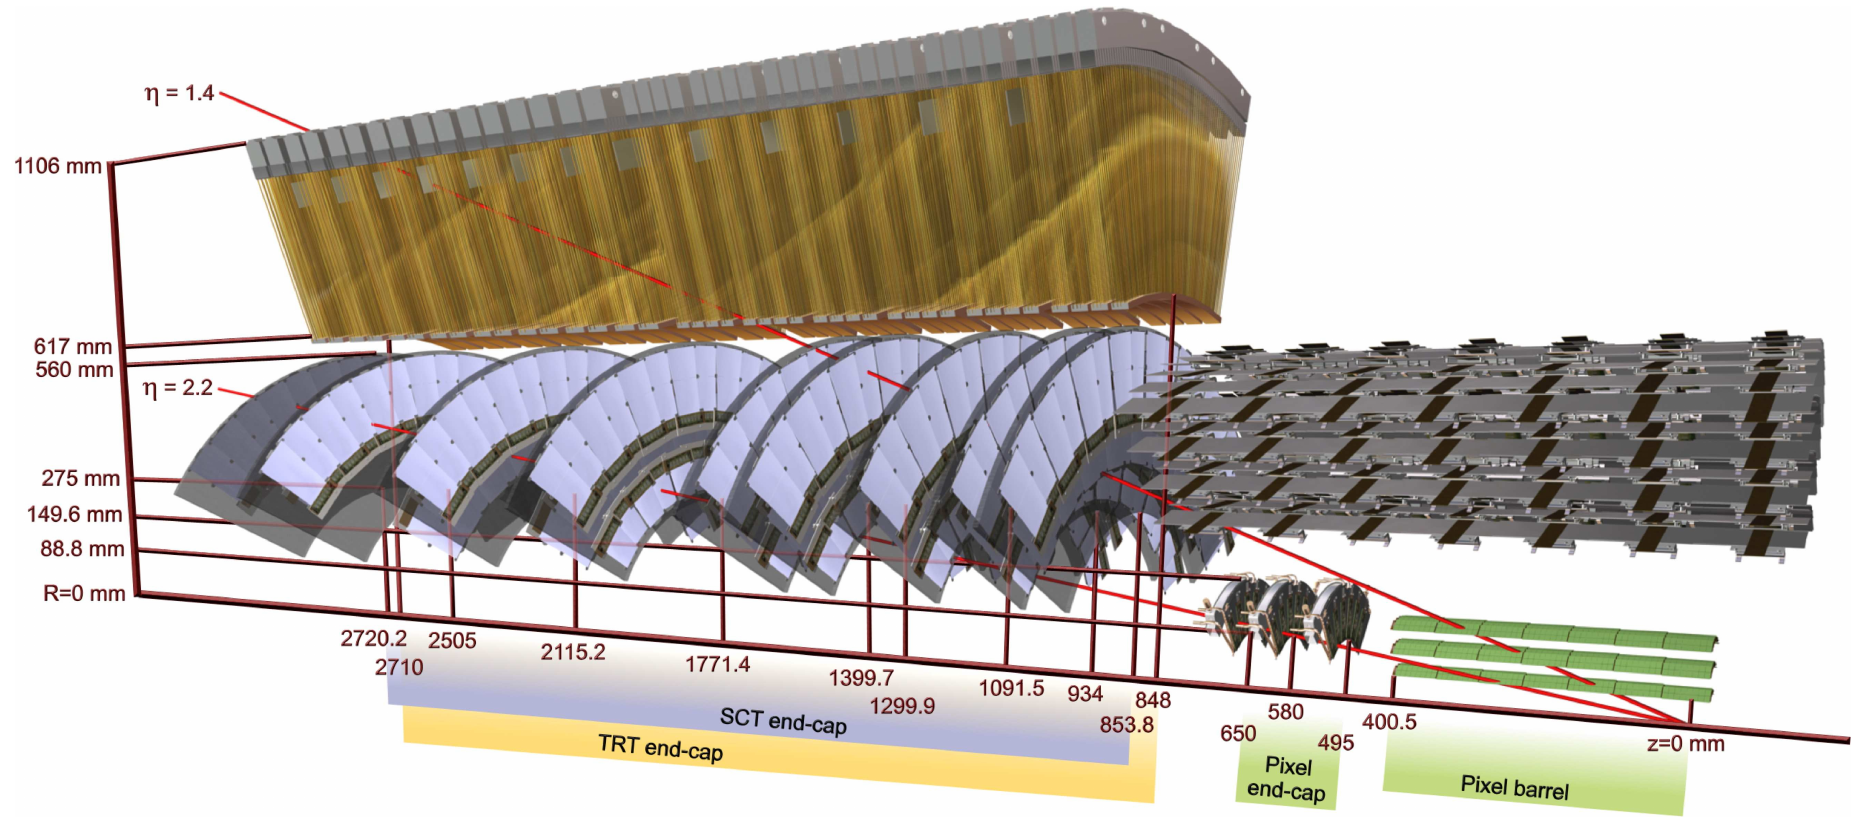
\includegraphics[width=\linewidth,height=\textheight,keepaspectratio]{atlas/inner_detector_endcap_measurements}
                    \caption{ID Endcap}
                    \label{fig:inner_detector_endcap_measurements}
                \end{subfigure}
                \begin{subfigure}{.48\textwidth}
                    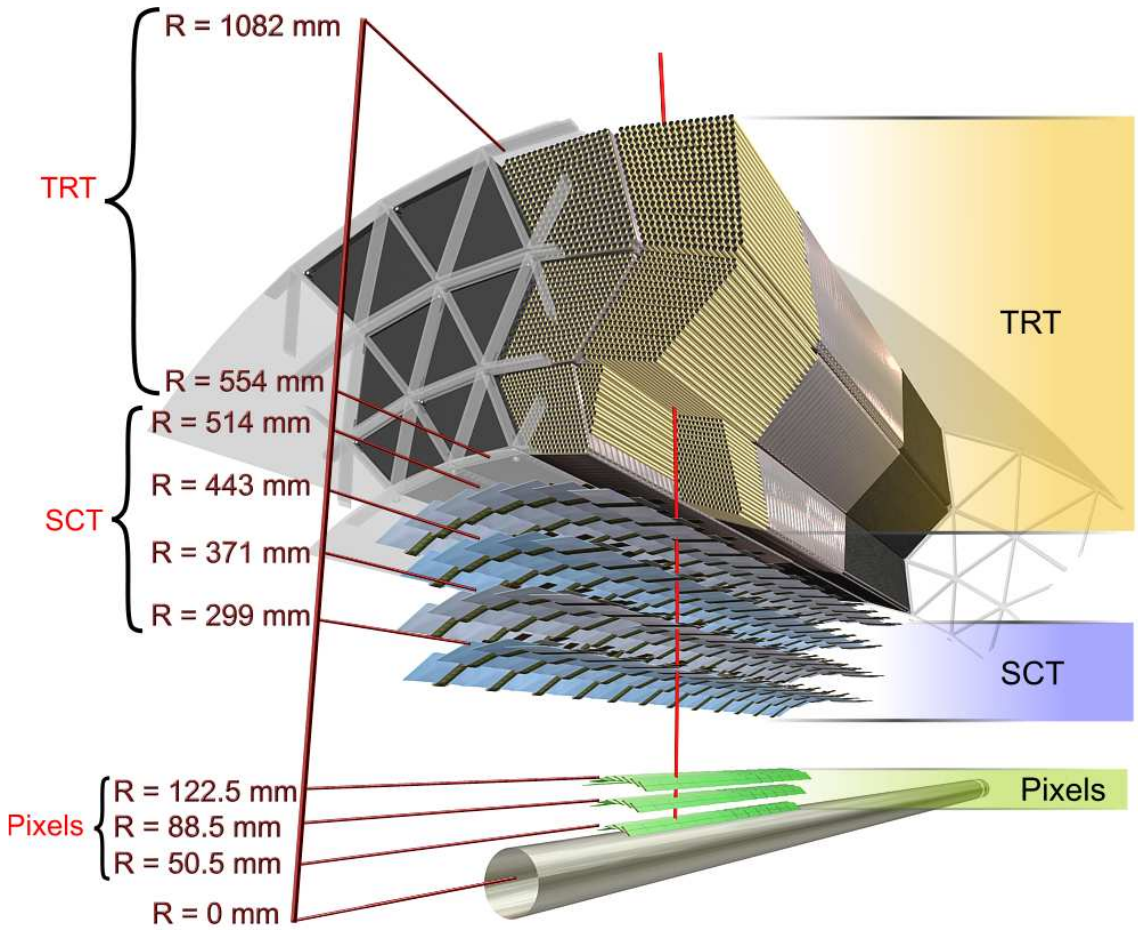
\includegraphics[width=\linewidth,height=\textheight,keepaspectratio]{atlas/inner_detector_barrel_measurements}
                    \caption{ID Barrel}
                    \label{fig:inner_detector_barrel_measurements}
                \end{subfigure}
                \caption{Visualization of the Inner Detector modules with corresponding measurements \cite{atlas_tdr}}
                \label{fig:inner_detector_measurements}
            \end{figure}

            For the TRT barrel, there are 52,544 straws 144 cm in length, while the endcaps each contain 122,880 straws 37 cm in length.
            These straws are arranged parallel to the beampipe in the barrel, and orthogonal to the beampipe in the endcap (see figure \ref{fig:inner_detector_measurements}).
            This arrangement is to maximize the number of straws traversed by an outgoing particle, typically 35-40 straws for $0 < |\eta| < 2$.
            Though each individual hit has a relatively low spatial resolution compared to the semiconductor detectors, the large number of hits compensates for this with a reduced statistical uncertainty.

            In addition to providing additional tracking information, the TRT provides a secondary purpose of aiding in the identification of electrons by means of detecting transition radiation. 
            Transition radiation is a phenomenon in which radiation is emitted when a charged particle crosses a boundary between two materials \cite{transition_radiation}.
            The TRT uses polypropylene as its transition radiation material, which is interleaved between the layers of straws.
            In the barrel, there are 73 layers of straws interwoven with polypropylene fibres, and in the endcaps there are 160 layers of straws with polypropylene foil between them.
            The large number of layers provide ample and repeated opportunity for charged particles crossing the TRT to encounter transition layers and emit identifying radiation, which is later used to distinguish electrons from other ionizing radiation.


\section{Calorimetry} \label{sec:calorimeter}
    The ATLAS Calorimeter system is designed to measure the energy of particles emerging from the Interaction Region.
    The entire collection of sub-detectors extends from the immediate outer edge of the Inner Detector region, out to a radius of 4.25 m, and longitudinally out to 6.12 m.
    Together the various systems achieve complete measurement coverage out to $|\eta| < 4.9$.

    There are a number of different ways to measure the energy of a particle, but in ATLAS this is done exclusively using the class of calorimeters known as \textit{sampling} calorimeters.
    Fundamentally, particle calorimeters work by impeding the path of a particle with some material, such that the particle is forced to interact with that material and deposit energy into it.
    This interaction must be such that it produces a measurable response, proportional to the deposited energy.
    A sampling calorimeter functions by measuring only a fraction of the deposited energy, spread out across the detector medium; i.e.\ by taking a sample of the energy.
    To do this, two different materials are used in the detector's construction, referred to as the active and inactive materials.
    The active material is the material which actually measures the energy of particles, using the same or similar techniques as the tracking systems discussed earlier.
    The inactive material in turn has no detection capabilities, but instead exists purely for the purpose of the aforementioned impedance of particle trajectories.
    Typically, inactive calorimeter material is a very dense and heavy high $Z$ medium, in order to maximize the number of particle interactions per unit distance.
    The active and inactive materials are arranged in alternating layers, so that the active material gets a snapshot of the way the particle is depositing energy across the entire length of the detector.\cite{energy_measurement}

    \begin{figure}
        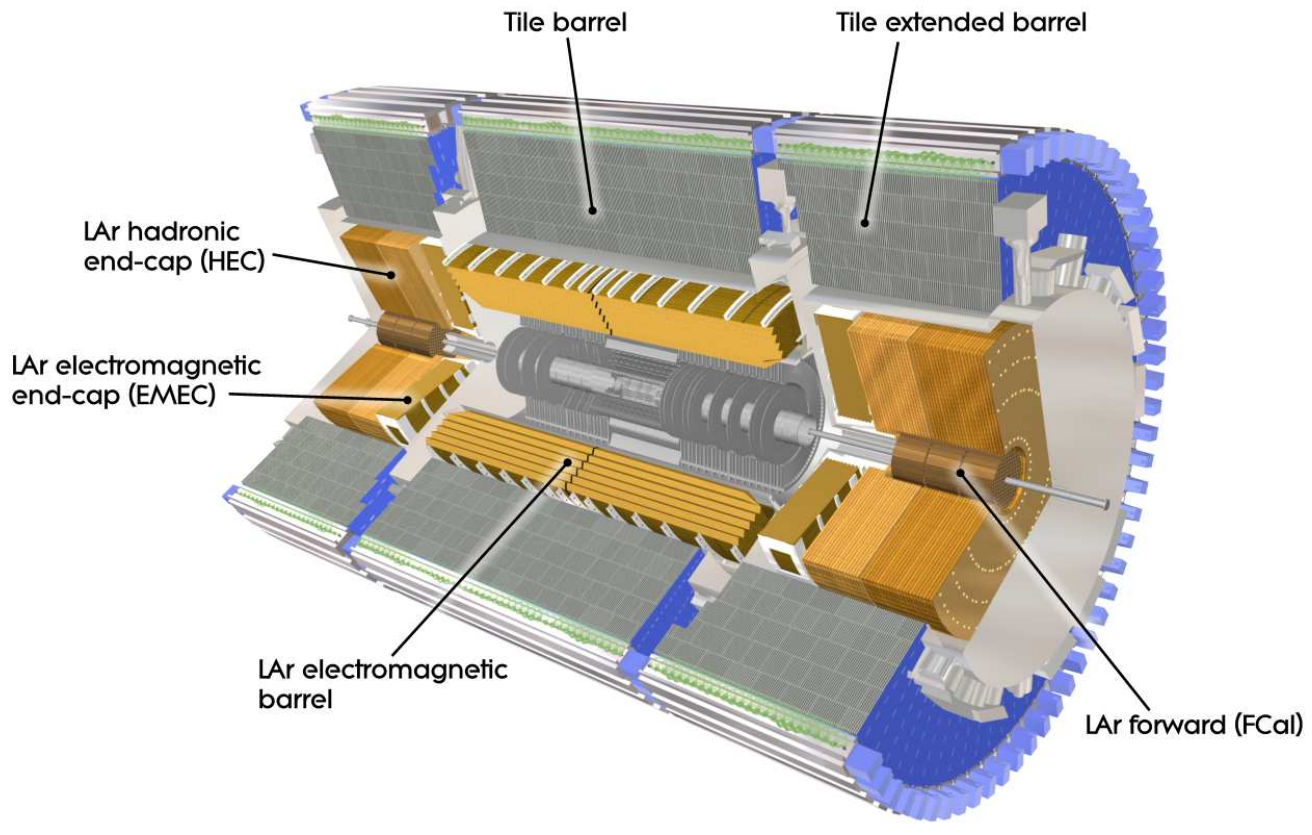
\includegraphics[width=\linewidth,height=\textheight,keepaspectratio]{atlas/cal_xsec}
        \caption{Cutaway view of the Calorimetry sub-system \cite{atlas_tdr}}
        \label{fig:cal_xsec}
    \end{figure}

    The Calorimetry system is split among three different subsystems, designed to measure two distinct kinds of particles.
    The innermost of these subsystems is the Electromagnetic Calorimeter (ECal), designed primarily to measure (anti) electrons and photons \cite{calorimetry_lecture}.
    These particles readily interact electromagnetically in the calorimeter material, rapidly losing energy and permitting the ECal to be more compact.
    Surrounding the ECal are the Hadronic Calorimeter (HCal) systems.
    These detectors, as their name suggests, detect hadrons, such as neutrons or pions.
    Not only are these particles heavier, but many of them are electrically neutral and can therefore only be stopped through repeated nuclear interactions \cite{energy_measurement}.
    Consequently, the HCal systems must be much thicker than the ECal systems(see figure \ref{fig:cal_rad_length}).
    \begin{figure}
        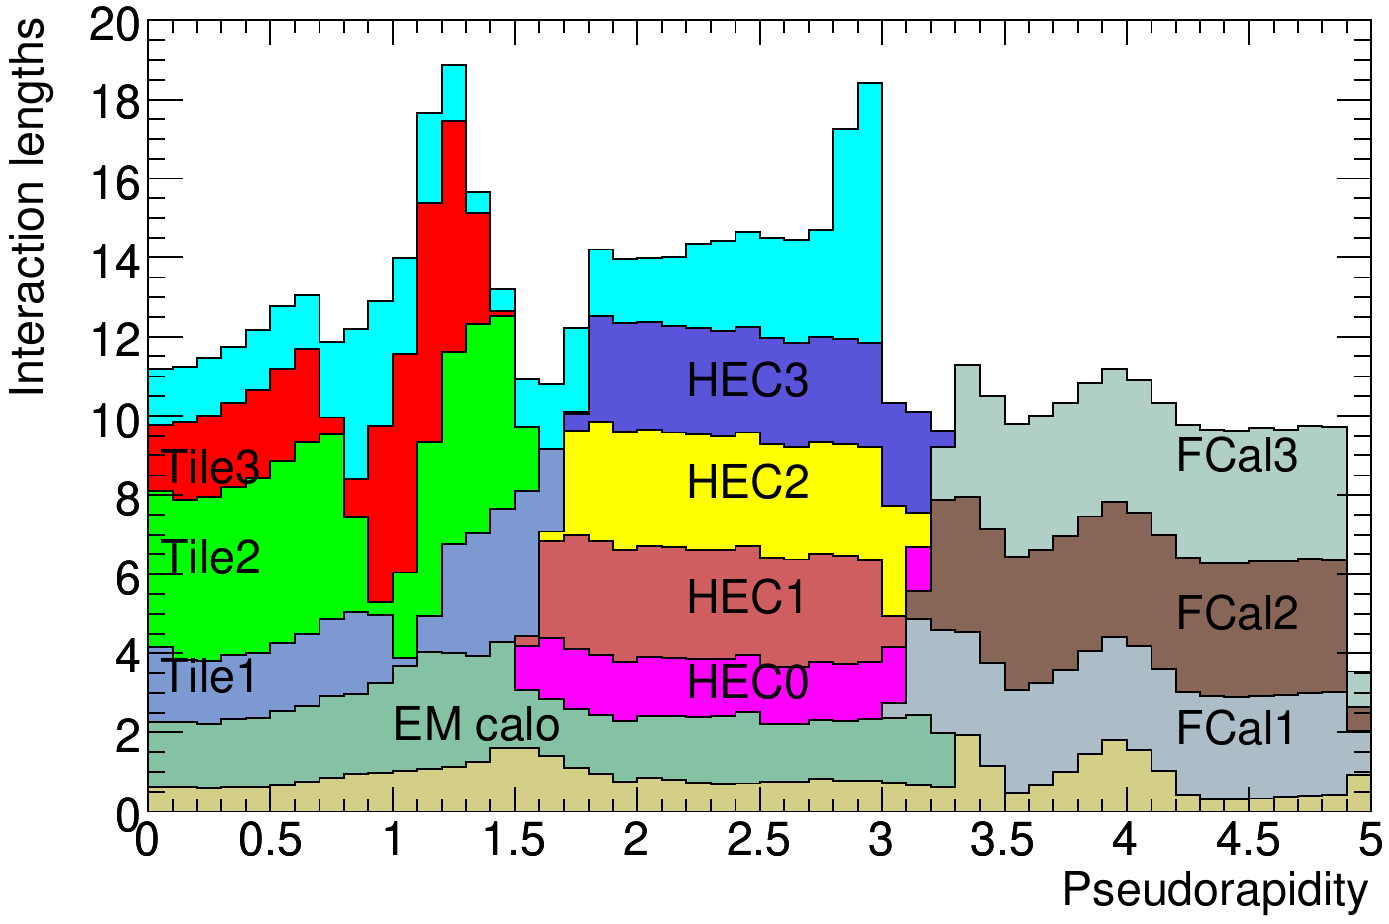
\includegraphics[width=\linewidth,height=\textheight,keepaspectratio]{atlas/cal_rad_length}
        \caption{Histogram of interaction lengths $X_0$ as a function of $\eta$ for the different sub-detectors \cite{atlas_tdr}}
        \label{fig:cal_rad_length}
    \end{figure}
    Additionally, they serve the role of preventing hadrons from escaping into the Muon Spectrometer.
    The final subsystem of the Calorimetry system is the Forward Calorimeter (FCal).
    The FCal records, across different sections, the energy of both electromagnetic and hadronic particles.
    It is constructed very close to the beampipe, and serves to extend the calorimetric measurement coverage out to an $|\eta|$ of 4.9.

    \subsection{Electromagnetic Calorimeters}
        Light, electromagnetically interacting particles, namely electrons/positrons and photons, are much more easily stopped than heavy or neutral particles.
        As these kinds of particles are the first to be stopped, the calorimeter responsible for measuring their energy, the Electromagnetic Calorimeter (ECal) is the closest to the IR.
        Furthermore, the lesser amount of material required for this detector permits higher resolution in its construction.
        In $\eta$, this resolution increase is a strict numerical change of 0.025 for ECal versus 0.1 for HCal (see table \ref{tab:cal_specs}).
        In $\phi$ though, the resolution is increased using a more creative geometry.
        Rather than simple flat plates, the active and inactive materials of the ECal are arranged in a unique ``accordion" design, in order to provide complete coverage in $\phi$.
        Additionally, while the ECal is unable to stop hadrons, it can still make measurements of such particles as they pass through it.
        Hence the ECal's secondary purpose of assisting the HCal with preliminary hadronic energy measurement.

        Due to its density, lead is used as the inactive material in both the ECal barrel and endcaps.
        For the active material, care must be taken to ensure the material and electronics provide both a linear ionization response, as well as the ability to withstand the radiation flux present this close to the IR.
        The material of choice for this situation has accordingly been chosen as liquid argon (LAr) \cite{Lar_cal_tdr}.
        These liquid argon calorimeters, used in the ECal and elsewhere, detect ionization from incident particles via capacitive coupling to electrodes placed outside the active LAr medium.

        Finally, the main layers of the ECal are augmented by a ``Presampler" placed in front of the ECal.
        An excess of support structure material exists in front of the ECal which absorbs a non-negligible amount of energy from traversing particles.
        The Presampler then acts to measure some the particles' energy before passing through this support material, so that this loss can be accounted for.

    \subsection{Hadronic Calorimeter}
        With lighter electromagnetic radiation already measured by the ECal, the Hadronic Calorimeter (HCal) has the task of measuring the energy of the particles (mostly hadrons) that remain.
        The more massive, often neutral, nature of these particles requires significantly more material to properly contain.
        As the Muon Spectrometer is dependent on observation of \textit{only} muons, the HCal's containment of hadrons is crucial not only to its own energy measurements, but also for the measurements the Muon system will make.
        The endcap portion of the HCal, known as the Hadronic Endcap Calorimeter (HEC), uses liquid argon for the active material, like the ECal, but uses copper plates for the inactive material.

        Distinct from the LAr-based calorimeters, the HCal Barrel and Extended Barrel must provide coverage to a very large area, making the LAr technology prohibitively costly.
        Referred to as the Tile Calorimeters, the HCal barrel system instead uses scintillating tiles as its active material, with steel plates as the inactive material.
        These tiles are less radiation resistant than the LAr sensors, but this is compensated by the Tile Calorimeter's larger distance from the IR.
        The scintillating tiles used in the Tile Calorimeter operate on different ionization detection principles than the other sensor technologies discussed so far.
        The key to scintillating materials is that they respond to ionizing radiation not by ion release, but by fluorescence.
        That is, when ionizing radiation crosses through the scintillation material, the atoms of the material momentarily enter an excited state.
        The excited material atoms promptly return to their base energy state, and release the excess energy in the form of ``scintillation light" photons.
        Ideally, this fluorescent response is related to the energy of the incident radiation through as linear a response as possible \cite{wiley_radiation_detection}.
        In the Tile Calorimeter, the scintillating material used is polystyrene, and the energy itself is measured by transferring the light to optical fibres located at the edge of the tile modules.
        These optical fibres direct the light to photomultiplier tubes (PMTs), which in turn convert the light to electrical signals to be read out \cite{tcal_tdr}.

    \subsection{Forward Calorimeter}
        The Forward Calorimeter (FCal) is the final sub-system of the ATLAS Calorimetry system, and acts to extend calorimetry coverage to the very forward detector region, out to $|\eta| < 4.9$.
        It is a single cylindrical block, but is divided into three sections, one behind the other.
        The innermost of these sections acts as an extension to the ECal, and the other two serve as forward HCal detectors.
        Due to their proximity to the IR and beam-line, all three use LAr for their active material, again for its radiation hardness.
        The main difference between the sections is that the electromagnetic section uses copper for its inactive material, while the hadronic components use tungsten \cite{Lar_cal_tdr}.

    \begin{table}[] \tiny \centering
\caption{General specifications of calorimeter systems \cite{atlas_tdr}.}
\label{tab:cal_specs}
\begin{tabular}{|l|lc|lc|}
\hline 
                                               &                  \multicolumn{2}{c|}{\textbf{Barrel}}            &           \multicolumn{2}{c|}{\textbf{End-cap}}                                 \\
\hline 
                                               \multicolumn{5}{|c|}{\textbf{EM Calorimeter}} \\
\hline 
                                               \multicolumn{5}{|c|}{Number of layers and $|\eta|$ coverage} \\
\hline 
Presampler                                     & 1                 & $|\eta|$ < 1.52                 & 1                               & 1.5 < $|\eta|$ < 1.8     \\
Calorimeter                                    & 3                 & $|\eta|$ < 1.35                 & 2                               & 1.375 < $|\eta|$ < 1.5   \\
                                               & 2                 & 1.35 < $|\eta|$ < 1.475 & 3                                       & 1.5 < $|\eta|$ < 2.5     \\
                                               &                   &                                 & 2                            & 2.5 < $|\eta|$ < 3.2     \\
\hline 
                                               \multicolumn{5}{|c|}{Granularity $\Delta \eta \times \Delta \phi$ versus $|\eta|$} \\
\hline 
Presampler                                     & 0.025 × 0.1       & $|\eta|$ < 1.52                 & 0.025 × 0.1                     & 1.5 < $|\eta|$ < 1.8     \\
Calorimeter 1st layer                          & 0.025/8 × 0.1     & $|\eta|$ < 1.40                 & 0.050 × 0.1                     & 1.375 < $|\eta|$ < 1.425 \\
                                               & 0.025 × 0.025     & 1.40 < $|\eta|$ < 1.475 & 0.025 × 0.1                             & 1.425 < $|\eta|$ < 1.5   \\
                                               &                   &                                    & 0.025/8 × 0.1                   & 1.5 < $|\eta|$ < 1.8     \\
                                               &                   &                                    & 0.025/6 × 0.1                   & 1.8 < $|\eta|$ < 2.0     \\
                                               &                   &                                    & 0.025/4 × 0.1                   & 2.0 < $|\eta|$ < 2.4     \\
                                               &                   &                                    & 0.025 × 0.1                     & 2.4 < $|\eta|$ < 2.5     \\
                                               &                   &                                    & 0.1 × 0.1                       & 2.5 < $|\eta|$ < 3.2     \\
\hline 
Calorimeter 2nd layer                          & 0.025 × 0.025     & $|\eta|$ < 1.40                    & 0.050 × 0.025                   & 1.375 < $|\eta|$ < 1.425 \\
                                               & 0.075 × 0.025     & 1.40 < $|\eta|$ < 1.475 & 0.025 × 0.025                              & 1.425 < $|\eta|$ < 2.5   \\
                                               &                   &                                    & 0.1 × 0.1                       & 2.5 < $|\eta|$ < 3.2     \\
\hline 
Calorimeter 3rd layer                          & 0.050 × 0.025     & $|\eta|$ < 1.35                 & 0.050 × 0.025                   & 1.5 < $|\eta|$ < 2.5     \\
\hline 
                                               \multicolumn{5}{|c|}{Number of readout channels} \\
\hline 
Presampler                                     & 7808              &                                    & 1536 (both sides)               &                                     \\
Calorimeter                                    & 101760            &                                    & 62208 (both sides)              &                                     \\
\hline 
                                               \multicolumn{5}{|c|}{\textbf{LAr Hadronic End-cap}} \\
\hline 
$|\eta|$ coverage                              &                   &                                    & 1.5 < $|\eta|$ < 3.2 &                                     \\
Number of layers                               &                   &                                    & 4                               &                                     \\
\hline 
Granularity $\Delta \eta \times \Delta \phi$   &                   &                                    & 0.1 × 0.1                       & 1.5 < $|\eta|$ < 2.5     \\
                                               &                   &                                    & 0.2 × 0.2                       & 2.5 < $|\eta|$ < 3.2     \\
\hline 
Readout channels                               &                   &                                    & 5632 (both sides)               &                                     \\
\hline 
                                                       \multicolumn{5}{|c|}{\textbf{LAr Forward Calorimeter}} \\
\hline 
$|\eta|$ coverage                              &                   &                                    & 3.1 < $|\eta|$ < 4.9 &                                     \\
Number of layers                               &                   &                                    & 3                               &                                     \\
\hline 
Granularity $\Delta x \times \Delta y$ (cm)    &                   &                                    & FCal1: 3.0 × 2.6                & 3.15 < $|\eta|$ < 4.30   \\
                                               &                   &                                    & FCal1: \~ four times finer       & 3.10 < $|\eta|$ < 3.15,  \\
                                               &                   &                                    &                                 & 4.30 < $|\eta|$ < 4.83   \\
                                               &                   &                                    & FCal2: 3.3 × 4.2                & 3.24 < $|\eta|$ < 4.50   \\
                                               &                   &                                    & FCal2: \~ four times finer       & 3.20 < $|\eta|$ < 3.24,  \\
                                               &                   &                                    &                                 & 4.50 < $|\eta|$ < 4.81   \\
                                               &                   &                                    & FCal3: 5.4 × 4.7                & 3.32 < $|\eta|$ < 4.60   \\
                                               &                   &                                    & FCal3: \~ four times finer       & 3.29 < $|\eta|$ < 3.32,  \\
                                               &                   &                                    &                                 & 4.60 < $|\eta|$ < 4.75   \\
\hline 
Readout channels                               &                   &                                    & 3524 (both sides)               &                                     \\
\hline 
                                               \multicolumn{5}{|c|}{\textbf{Scintillator Tile Calorimeter}} \\
\hline 
                                               & Barrel            &                                    & Extended barrel                 &                                     \\
\hline 
$|\eta|$ coverage                              &    $|\eta|$ < 1.0 &                                    & 0.8 < $|\eta|$ < 1.7 &                                     \\
Number of layers                               & 3                 &                                    & 3                               &                                     \\
\hline 
Granularity $\Delta \eta \times \Delta \phi$   & 0.1 × 0.1         &                                    & 0.1 × 0.1                       &                                     \\
Last layer                                     & 0.2 × 0.1         &                                    & 0.2 × 0.1                       &                                     \\
\hline 
Readout channels                               & 5760              &                                    & 4092 (both sides)               &                                    \\
\hline 
\end{tabular} \end{table}



\section{Muon Spectrometer} \label{sec:muon}
    Far from the interaction region, beyond all other sub-systems, lies the Muon Spectrometer.
    Muons interact electromagnetically and carry charge, as electrons, but their much higher mass vastly suppresses their differential energy deposition \cite{wiley_radiation_detection}.
    As well, they do not interact through the strong force, and so are completely unaffected by nuclear interactions.
    For these reasons, muons pass almost unfazed through the entire ATLAS Calorimetry system.
    Moreover, their large mass and high momentum means they are barely deflected by the Inner Detector's solenoid magnet, leaving the details of their momentum unknown.
    It thus falls to the Muon Spectrometer to provide this critical information of muon momentum, which all the other sensors are unable to deliver.

    The Muon Spectrometer system is immense.
    The Muon barrels start at a radii of 5 m from the beam axis and extend all the way out to 10 m.
    The endcaps start at a $|z|$ of roughly 7.4 m, and proceed to an extent of 21.5 m.
    Such size poses a challenge, as the Muon system must provide tracking across its entire volume.
    %Its distance from the interaction point ameliorates this issue though, as it permits the Muon detectors to operate at much lower spatial resultions than the inner detectors, while still retaining similar anngular resolution.
    To achieve this goal, the Muon system is split into two primary sections, the Precision Track Chambers and the Trigger Chambers.
    The Precision Track Chambers are primarily responsible for providing tracking of muons leaving the ATLAS detector volume in order to determine their momentum.
    Past the Precision Track Chamber are the Trigger Chambers, which are primarily designed for providing rapid information of muon track multiplicity and energy range, used in large part by the trigger system.

    \begin{figure}
        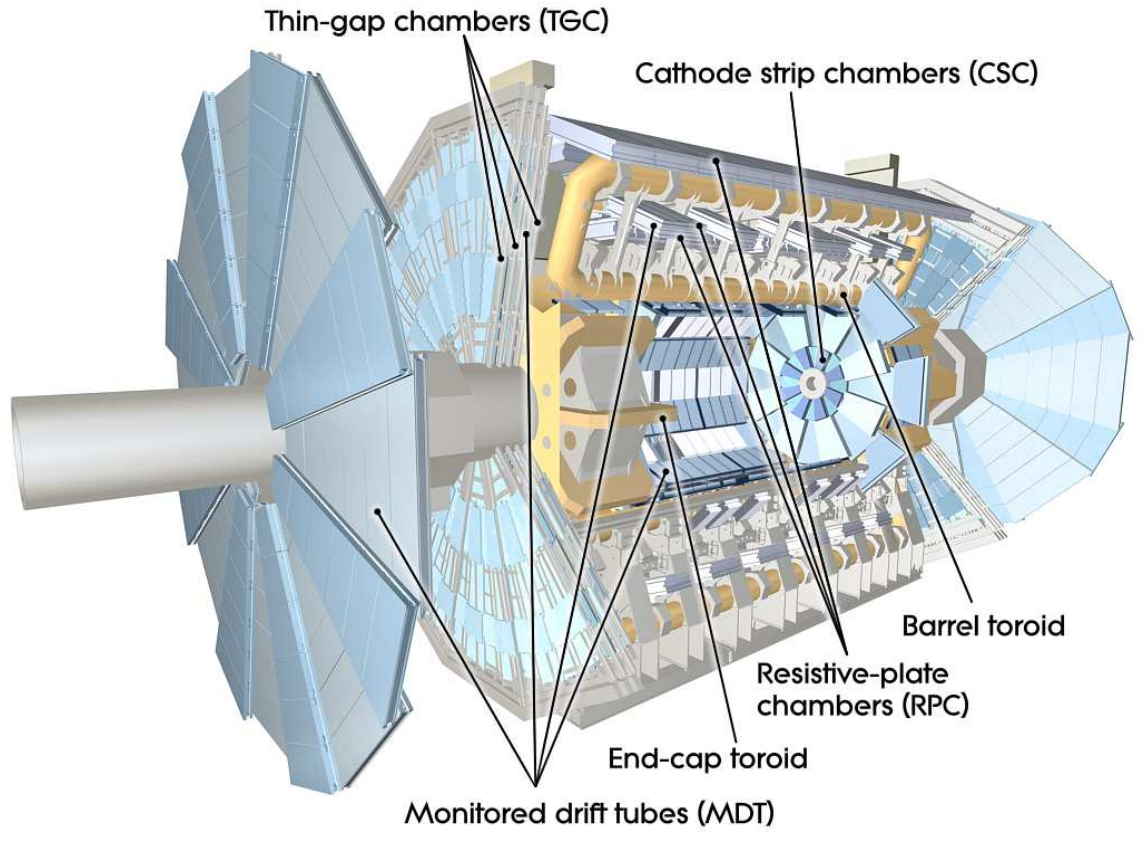
\includegraphics[width=\linewidth,height=\textheight,keepaspectratio]{atlas/muon_xsec}
        \caption{Cutaway view of the Muon Spectrometer \cite{atlas_tdr}}
        \label{fig:muon_xsec}
    \end{figure}

    \subsection{Precision Track Chambers}
        The Precision Track Chambers are designed to provide high resolution measurements of track position and momentum for muons escaping the ATLAS detector. 
        As was done earlier in the Inner Detector system, this is achieved by applying a powerful magnetic field to the detector region in order to bend the muon tracks.
        Where the Inner Detector used a relatively small solenoid magnet for this purpose, the Muon system uses a much larger set of three air-core toroid magnets.
        These toroids are able to provide 1.5-5.5 Tm (Tesla-meters???) of bending power in the barrel region $0<|\eta|<1.4$, and 1-7.5 Tm in the endcap regions of $1.6<|\eta|<2.7$.
        Notably, the bending power is lower in the region where the fields overlap ($1.4<|\eta|<1.6$) \cite{atlas_tdr}.

        The Precision Track Chambers consist of two distinct detector technologies, the Monitored Drift Tube Chambers (MDTs) and Cathode-Strip Chambers (CSCs).
        Most of the Track Chambers' volume is made up of the MDTs, which are drift tube chambers (like the earlier TRT, but larger) filled with Ar/CO\textsubscript{2} gas using a tungsten-rhenium wire for charge collection.
        These are used in both the barrel and endcap regions, covering the range $|\eta| < 2.7$.
        The MDT consists of three endcap and three barrel layers, with a notable exception in the endcap region $2 < |\eta| < 2.7$.
        Within this $\eta$ range, for the first layer, the muon track density exceeds the resolution capabilities of the MDT's.
        This very specific $\eta$ range of this one particular endcap layer is where the CSC is used for tracking instead.
        The CSC's are multiwire drift chambers, meaning that the (gold-plated tungsten) anode wires do not each have their own individual drift tube.
        Instead, each of the many drift chambers contains many anodes and many cathode strips, made of copper.
        These chambers can read both coordinates of a track simultaneously, preventing the ambiguities that can occur if more than one track is present in the same chamber \cite{atlas_tdr}.

    \subsection{Trigger Chambers}\label{sec:muon-trigger_chamber}
        The last set of sensors in the ATLAS detector, the Trigger Chambers of the Muon system act to augment the information obtained from the Precision Track Chambers, as well as provide additional rapid information for the trigger system.
        It provides coverage in the range $|\eta| < 2.4$, only slightly less than that of the Track Chambers.
        The barrel and end-cap use two different technologies, Resistive Plate Chambers (RPCs) in the barrel, and Thin Gap Chambers (TGCs) in the endcaps.
        Both technologies are designed with extremely fast signal response times (15-25 ns) so that their measurements can be used to tag individual-beam crossings.
        %ok but why different techs?
        RPCs follow the same principle of operation as drift tube chambers, but the anode and cathodes are both conductive plates that maintain an electric potential in the gaseous mixture between them.
        The TGCs are multi-wire drift tube chambers with very small gaps between the anode wires and the cathode strips; indeed, the anode-cathode gaps are 1.4 mm are smaller than the anode-anode gaps of 1.8 mm.

    \begin{table}[hb] \centering \scriptsize
\caption{General specifications of the Muon Spectrometer \cite{atlas_tdr}.}
\label{tab:muon_specs}
\begin{tabular}{|l|l|}
\hline
\textbf{Monitored Drift Tubes}    & \textbf{MDT}                                                      \\
- Coverage               & $|\eta|$ < 2.7 (innermost layer: $|\eta|$ < 2.0)         \\
- Number of chambers     & 1088 (1150)                                              \\
- Number of channels     & 339 000 (354 000)                                        \\
- Function               & Precision tracking                                       \\
\hline
\textbf{Cathode Strip Chambers}   & \textbf{CSC}                                                      \\
- Coverage               & 2.0 < $|\eta|$ < 2.7                                     \\
- Number of chambers     & 32                                                       \\
- Number of channels     & 31 000                                                   \\
- Function               & Precision tracking                                       \\
\hline
\textbf{Resistive Plate Chambers} & \textbf{RPC}                                                      \\
- Coverage               & $|\eta|$ < 1.05                                          \\
- Number of chambers     & 544 (606)                                                \\
- Number of channels     & 359 000 (373 000)                                        \\
- Function               & Triggering, second coordinate                            \\
\hline
\textbf{Thin Gap Chambers}        & \textbf{TGC}                                                      \\
- Coverage               & 1.05 < $|\eta|$ < 2.7 (2.4 for triggering)               \\
- Number of chambers     & 3588                                                     \\
- Number of channels     & 318 000                                                  \\
- Function               & Triggering, second coordinate                            \\
\hline
\end{tabular} \end{table}

